\documentclass[11pt,a4paper]{article}

\usepackage[margin=0.9in]{geometry}
\usepackage{graphicx}
\usepackage{pdfpages}
\usepackage{booktabs}
\usepackage{float}
\usepackage{natbib}
\usepackage{newtxtext,newtxmath}
\usepackage[hidelinks]{hyperref}

\graphicspath{{./}}
\emergencystretch=2em

\title{Thieulot annulus Stokes benchmark}
\author{}
\date{}

\begin{document}

\maketitle
\vspace{-2.0em}

\section{Introduction}

The annulus benchmark of \citet{thieulot2018} provides an analytical solution for incompressible, isoviscous Stokes flow in a two-dimensional cylindrical shell. The benchmark is designed for geodynamic Stokes solvers because it combines curved boundaries, a radial gravity field, non-trivial density forcing, and a velocity field that is tangential on both the inner and outer boundaries. The integer parameter \(k\) controls the number of convection cells and therefore provides a simple way to increase the angular complexity of the manufactured solution.

Here we use this benchmark to verify the Underworld3 annulus Stokes implementation. The calculations use the analytical density, velocity, and pressure fields of \citet{thieulot2018}; relative volume \(L_2\)-norm errors are evaluated for velocity and pressure, and boundary pressure profiles are compared directly against the analytical solution.

\section{Benchmark setup}

The model solves
\[
  -\nabla\cdot\boldsymbol{\sigma}=\rho\mathbf{g},
  \qquad
  \nabla\cdot\mathbf{u}=0,
\]
in an annulus with inner radius \(R_1=1\) and outer radius \(R_2=2\). The viscosity is constant and the gravity vector is radial. The analytical solution is parameterised by \(k\), with \(k=1,2,4\) shown for the field plots and boundary-pressure profiles, and \(k=1,4,8\) used for the convergence study. Mesh resolution is reported using the nominal cell size \(h\). The convergence calculations use the element pairs \(P_1\times P_0\), \(P_1\times P_1\), \(P_2\times P_1\), and \(P_3\times P_2\), allowing the expected order hierarchy of mixed finite-element approximations to be tested.

\section{Analytical fields}

\begin{figure}[H]
    \centering
    
\includegraphics[width=0.98\linewidth]{figure_1_thieulot_annulus_analytical.pdf}
    \caption{Analytical density, velocity, and pressure fields for the Thieulot annulus benchmark. Columns correspond to increasing \(k\), which increases the number of convection cells in the annulus.}
    \label{fig:thieulot_annulus_fields}
\end{figure}

Figure~\ref{fig:thieulot_annulus_fields} shows the forcing and analytical fields used in the verification runs. Increasing \(k\) increases the azimuthal wavenumber of the solution, producing progressively finer angular structure in density, velocity, and pressure. These fields are useful visual diagnostics because the exact solution contains strong angular variation while maintaining tangential velocity on both curved boundaries.

\section{Velocity and pressure convergence}

\begin{figure}[H]
    \centering
    
\includegraphics[width=0.98\linewidth]{figure_5_thieulot_annulus_convergence.pdf}
    \caption{Convergence of relative volume \(L_2\)-norm velocity and pressure errors for the annulus Thieulot benchmark. Reference lines indicate the expected smooth-solution rates for the higher-order element pairs.}
    \label{fig:thieulot_annulus_convergence}
\end{figure}

For sufficiently smooth Stokes solutions, stable Taylor--Hood-type approximations are expected to converge with order \(p+1\) in the velocity \(L_2\) norm and order \(p\) in the pressure \(L_2\) norm for a \(P_{p+1}\times P_p\) pair, assuming that geometry and quadrature errors are not dominant \citep[e.g.][]{girault1986,boffi2013}. The UW3 results follow this pattern for the higher-order pairs. The \(P_2\times P_1\) calculations show approximately \(O(h^3)\) velocity convergence and \(O(h^2)\) pressure convergence for \(k=1,4,8\). The \(P_3\times P_2\) calculations show approximately \(O(h^4)\) velocity convergence and \(O(h^3)\) pressure convergence until the finest resolutions, where the velocity error approaches a small absolute error floor.

The lower-order element pairs behave as expected for less robust discretisations in this benchmark. The \(P_1\times P_1\) results show systematic velocity convergence close to \(O(h^2)\), while pressure convergence is lower and more variable. The \(P_1\times P_0\) results do not show useful convergence for this setup. This is consistent with the role of stable velocity--pressure coupling in incompressible Stokes discretisations and indicates that the higher-order Taylor--Hood pairs are the appropriate production choices for this benchmark.

\section{Tabulated errors}

The numerical values and pairwise convergence rates are provided in the following pages. Each table groups \(k=1,4,8\) and reports \(h\), velocity error, velocity rate, pressure error, and pressure rate for one element pair.

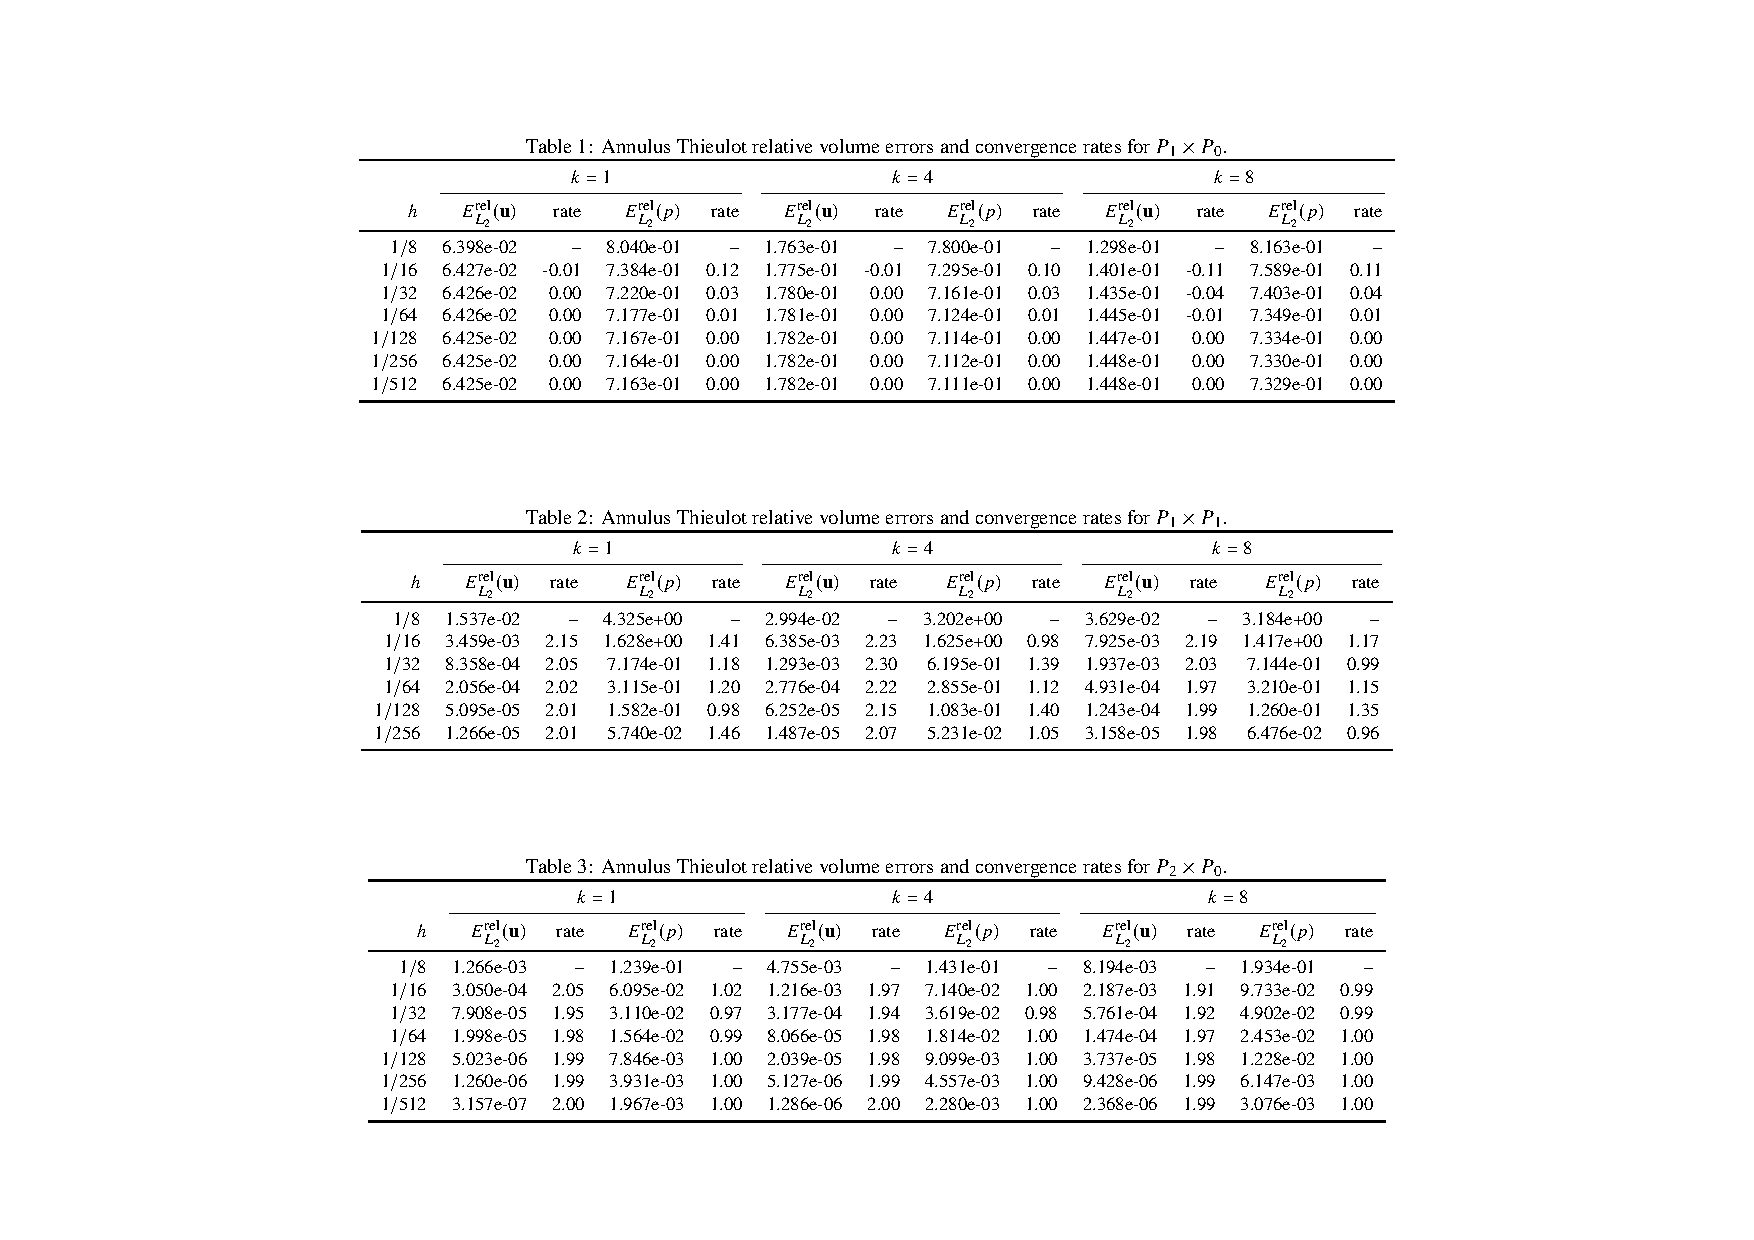
\includepdf[pages=-,fitpaper=true,pagecommand={\thispagestyle{plain}}]{table_figure_5_thieulot_annulus_convergence.pdf}

\section{Boundary pressure}

\begin{figure}[H]
    \centering
    
\includegraphics[width=0.92\linewidth]{figure_2_thieulot_annulus_pressure_boundary.pdf}
    \caption{Pressure along the inner and outer annulus boundaries for \(k=1,2,4\), using the \(h=1/128\) calculations. Solid curves denote the analytical solution and dashed curves denote UW3 values sampled from the numerical pressure field.}
    \label{fig:thieulot_annulus_boundary_pressure}
\end{figure}

Figure~\ref{fig:thieulot_annulus_boundary_pressure} reproduces the boundary-pressure comparison of \citet{thieulot2018} using the \(h=1/128\) UW3 models. The numerical curves are phase-aligned with the analytical pressure on both \(r=R_1\) and \(r=R_2\), and the amplitude agreement is close for all tested values of \(k\). This comparison is a complementary diagnostic to the volume \(L_2\) norms because it checks the pressure field directly on the curved boundaries, where geometric representation and pressure recovery errors are most visible.

\section{Discussion and conclusions}

The annulus Thieulot benchmark verifies the UW3 Stokes implementation for a smooth analytical solution in a curved two-dimensional shell. The analytical field plots confirm that the benchmark exercises non-trivial angular structure, and the convergence results demonstrate the expected finite-element hierarchy for the stable higher-order pairs. In particular, \(P_2\times P_1\) recovers approximately third-order velocity and second-order pressure convergence, while \(P_3\times P_2\) recovers approximately fourth-order velocity and third-order pressure convergence before fine-grid error-floor effects become visible.

The direct boundary-pressure comparison further indicates that the pressure solution is accurate not only in the volume norm but also on the annulus boundaries. Together, the convergence and boundary-profile results are consistent with the analytical benchmark behaviour reported by \citet{thieulot2018} and support the use of the annulus Thieulot problem as a production verification test for Underworld3 curved-domain Stokes calculations.

\bibliographystyle{plainnat}
\bibliography{thieulot_annulus_benchmark_report_refs}

\end{document}
